\subsection{Thiết kế giao diện người dùng}

Giao diện người dùng được thiết kế và triển khai hoàn toàn bằng Flutter với BLoC pattern, tuân thủ Material 3 Design, tối ưu cho thiết bị di động (iOS \& Android).

Các màn hình được prototype trên Figma (xem phụ lục C).

\subsubsection{Onboarding}

\begin{figure}[H]
    \centering
    \begin{subfigure}[b]{0.32\textwidth}
        \centering
        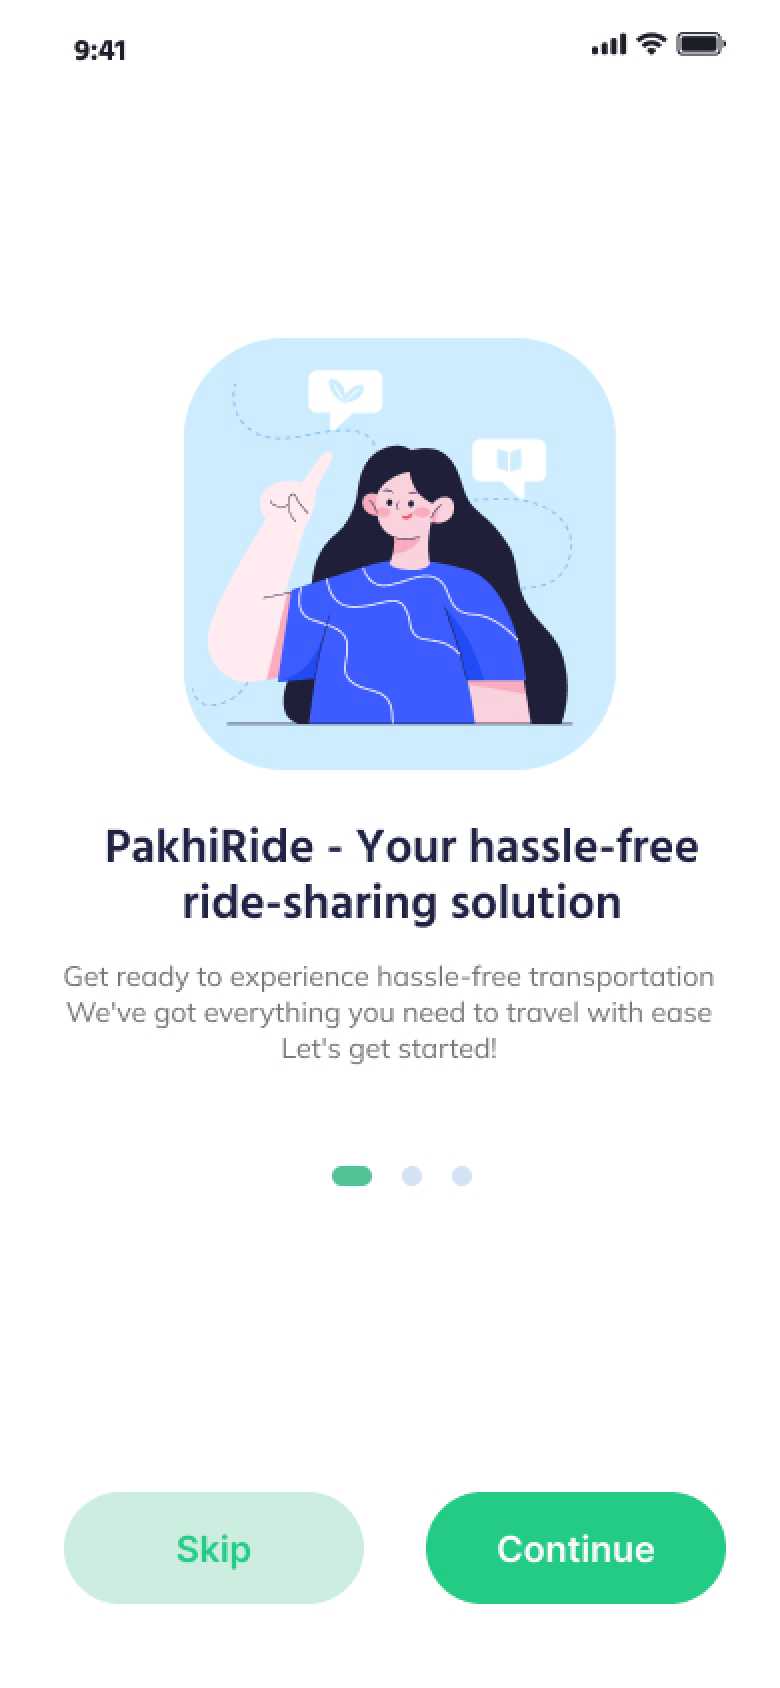
\includegraphics[width=\textwidth]{Images/Design/UIUX/onboard/ob1.png}
        \caption{Onboarding 1}
    \end{subfigure}
    \hfill
    \begin{subfigure}[b]{0.32\textwidth}
        \centering
        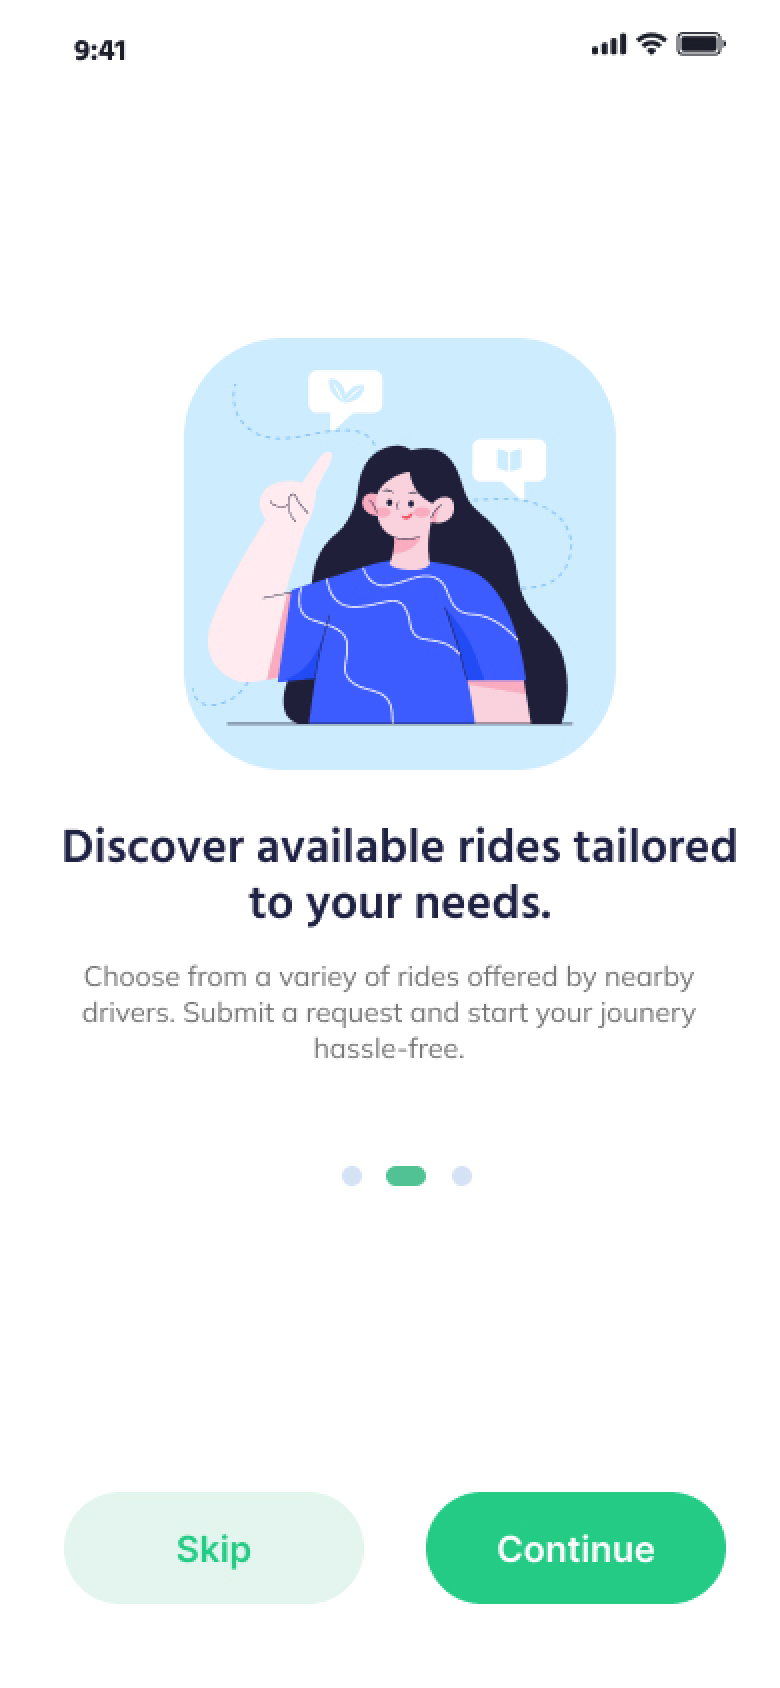
\includegraphics[width=\textwidth]{Images/Design/UIUX/onboard/ob2.png}
        \caption{Onboarding 2}
    \end{subfigure}
    \hfill
    \begin{subfigure}[b]{0.32\textwidth}
        \centering
        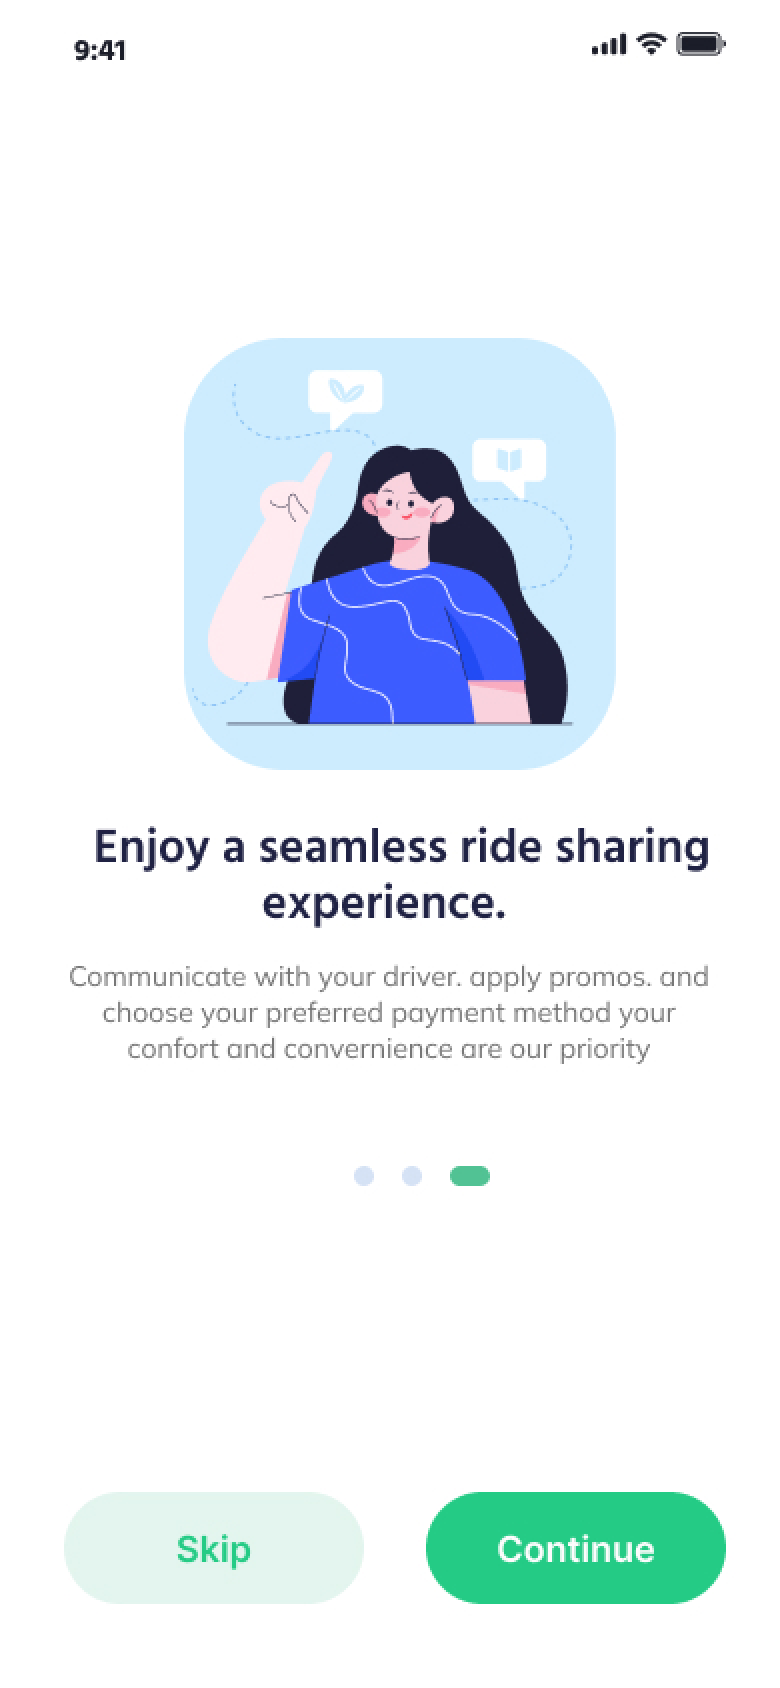
\includegraphics[width=\textwidth]{Images/Design/UIUX/onboard/ob3.png}
        \caption{Onboarding 3}
    \end{subfigure}
    \caption{Giao diện khởi tạo tài khoản (UC-01)}
    \label{fig:ui-onboard}
\end{figure}
Màn hình onboarding giới thiệu ngắn gọn mô hình chia sẻ P2P và lợi ích môi trường. 

\newpage
\subsubsection{Đăng nhập – Đăng ký}
\begin{figure}[H]
    \centering
    \begin{subfigure}[b]{0.32\textwidth}
        \centering
        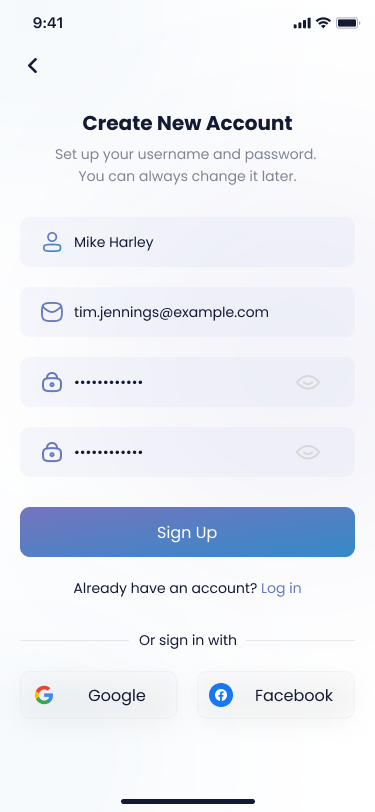
\includegraphics[width=\textwidth]{Images/Design/UIUX/auth/regis.png}
        \caption{Đăng ký}
    \end{subfigure}
    \hfill
    \begin{subfigure}[b]{0.32\textwidth}
        \centering
        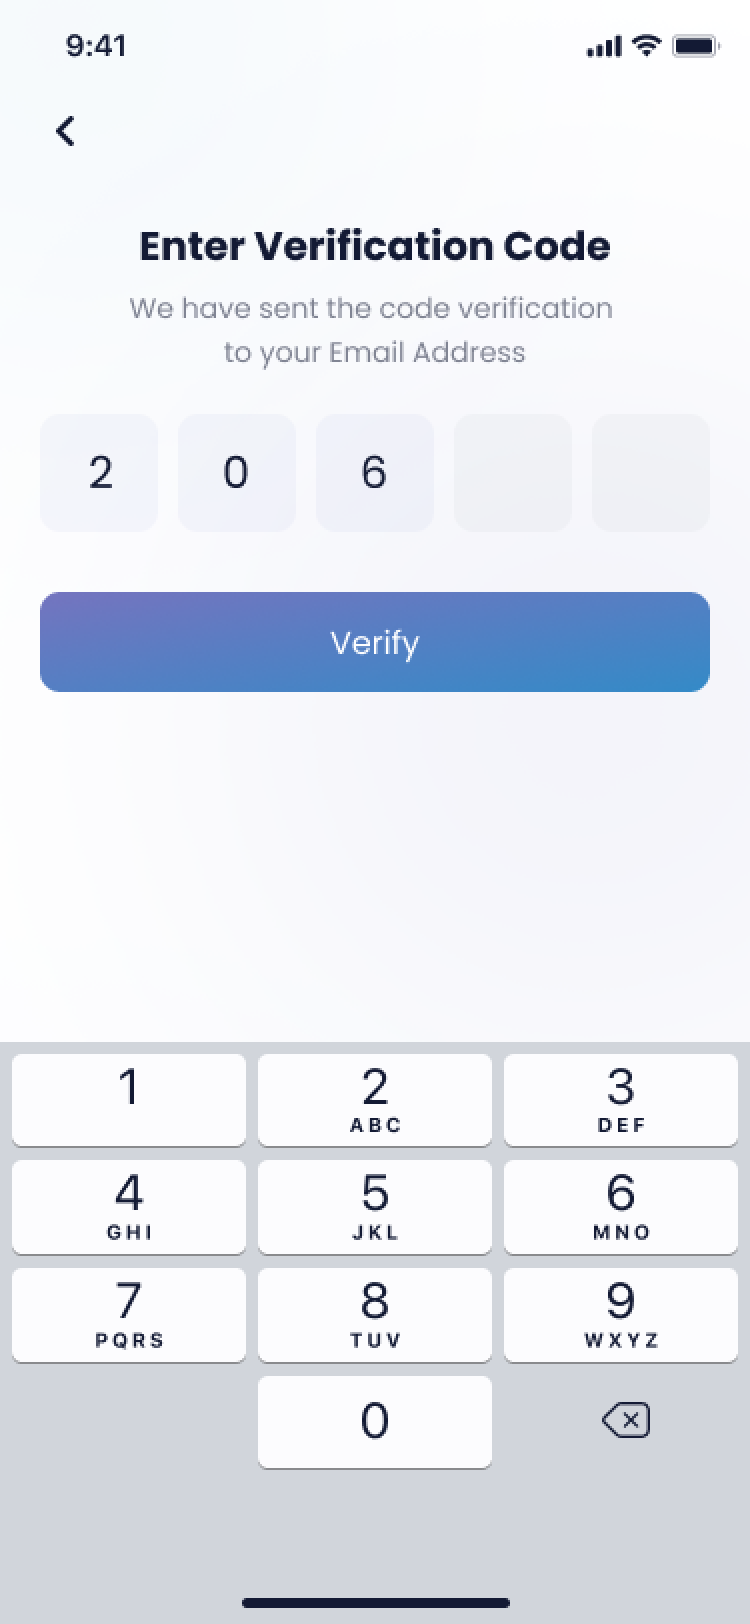
\includegraphics[width=\textwidth]{Images/Design/UIUX/auth/otp.png}
        \caption{OTP}
    \end{subfigure}
    \hfill
    \begin{subfigure}[b]{0.32\textwidth}
        \centering
        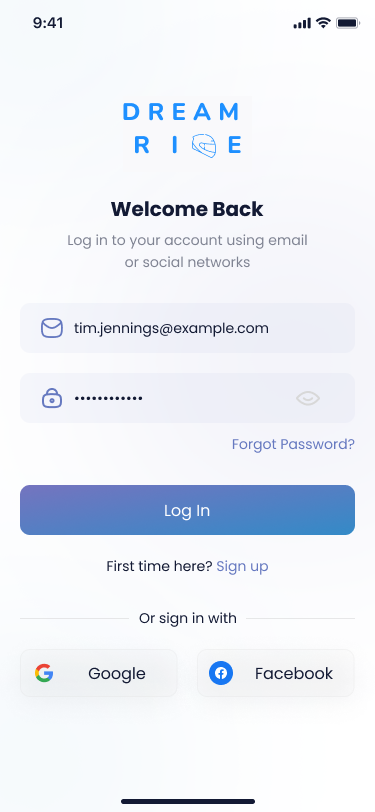
\includegraphics[width=\textwidth]{Images/Design/UIUX/auth/login.png}
        \caption{Đăng nhập}
    \end{subfigure}
    \caption{Giao diện khởi tạo tài khoản (UC-01)}
    \label{fig:ui-auth}
\end{figure}
Người dùng có thể đăng nhập nhanh bằng email/số điện thoại + OTP hoặc OAuth (Google/Zalo). Quy trình đăng ký yêu cầu xác minh CCCD và selfie để đảm bảo tính xác thực ngay từ đầu — yếu tố then chốt xây dựng niềm tin trong hệ thống chia sẻ ngang hàng. Giao diện tối giản, chỉ hiển thị một hành động chính tại một thời điểm, giảm tỷ lệ thoát người dùng mới.
\newpage

\subsubsection{Trang chủ \& Tìm kiếm xe}

\begin{figure}[H]
    \centering
    \begin{subfigure}[b]{0.32\textwidth}
        \centering
        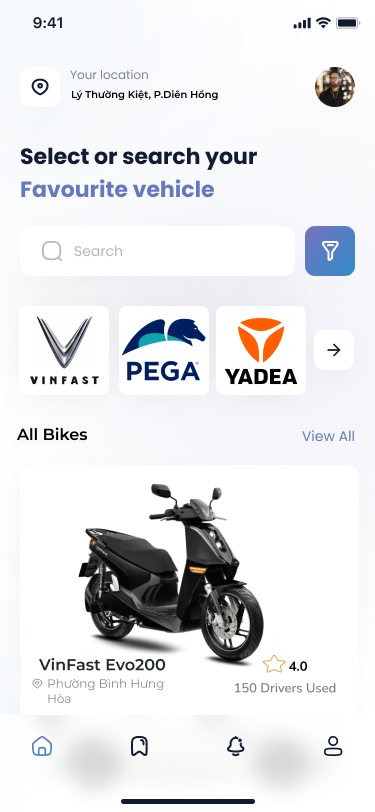
\includegraphics[width=\textwidth]{Images/Design/UIUX/Home/home.png}
        \caption{Home screen}
    \end{subfigure}
    \hfill
    \begin{subfigure}[b]{0.32\textwidth}
        \centering
        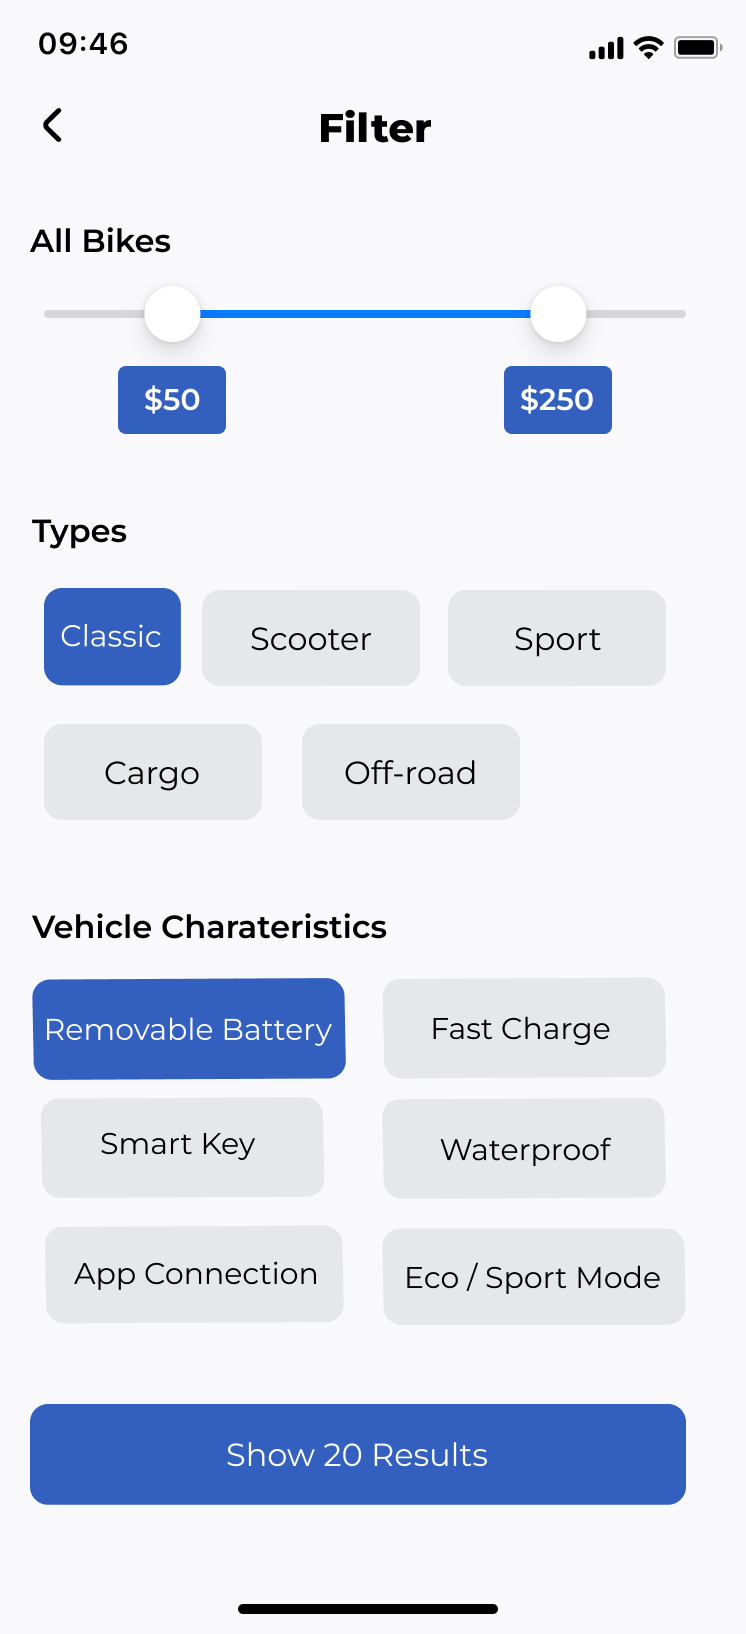
\includegraphics[width=\textwidth]{Images/Design/UIUX/Home/filter.png}
        \caption{Bộ lọc tìm kiếm}
    \end{subfigure}
    \hfill
    \begin{subfigure}[b]{0.32\textwidth}
        \centering
        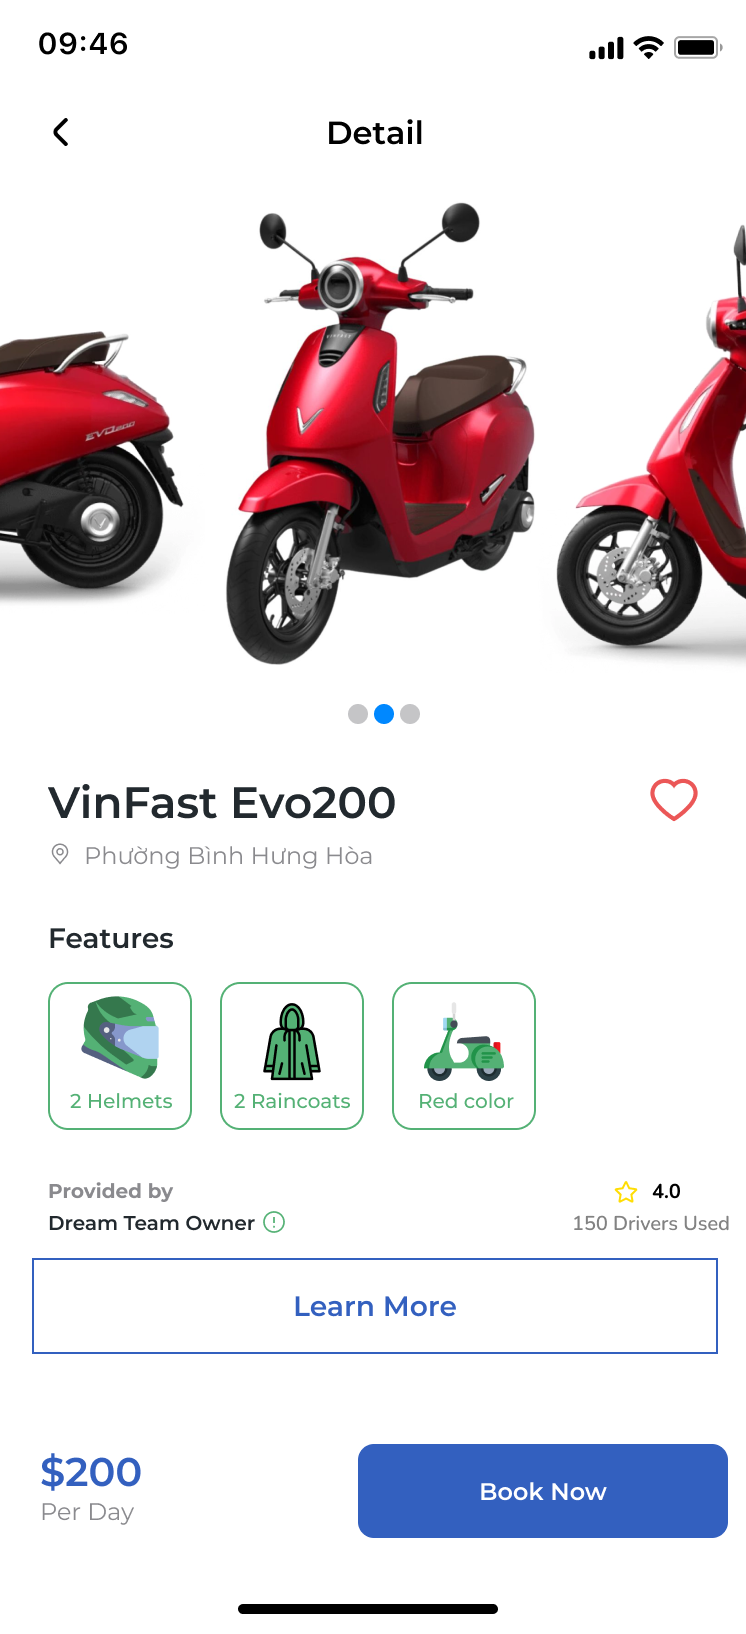
\includegraphics[width=\textwidth]{Images/Design/UIUX/Home/details.png}
        \caption{Chi tiết xe}
    \end{subfigure}
    \caption{Tìm kiếm và xem xe (UC-02, UC-03)}
    \label{fig:ui-search}
\end{figure}
Trang chủ hiển thị bản đồ Google Maps với các marker xe điện trong bán kính 3–5 km. Người dùng có thể kéo để thay đổi vùng tìm kiếm hoặc sử dụng bộ lọc nâng cao: mức pin $\geq 30\%$, giá/giờ, đánh giá chủ xe $\geq 4.0$, loại xe (VinFast Feliz, Yadea, DatBike...).
Màn hình chi tiết xe hiển thị hình ảnh thực tế, thông tin chủ xe (avatar, trust score), lịch sử đánh giá và nút “Đặt thuê ngay”. Thiết kế ưu tiên hình ảnh lớn và thông tin quan trọng ở vùng thumb zone.
\newpage
\subsubsection{Đặt thuê \& Thanh toán}

\begin{figure}[H]
    \centering
    \begin{subfigure}[b]{0.32\textwidth}
        \centering
        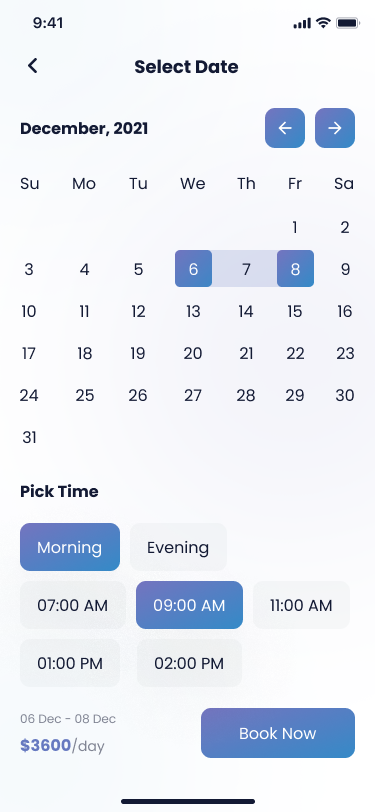
\includegraphics[width=\textwidth]{Images/Design/UIUX/renter/date.png}
        \caption{Chọn thời gian thuê}
    \end{subfigure}
    \hfill
    \begin{subfigure}[b]{0.32\textwidth}
        \centering
        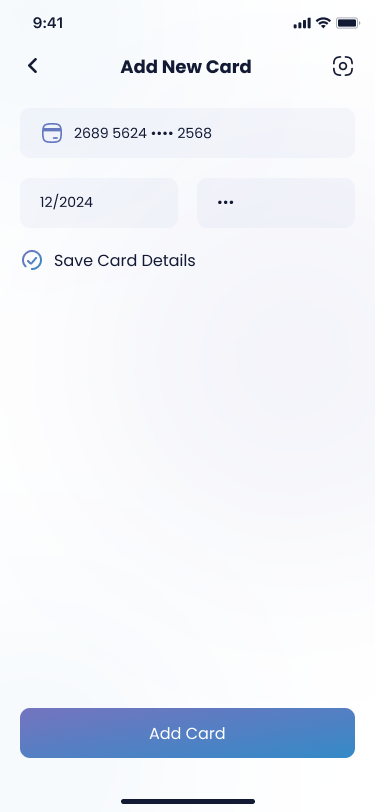
\includegraphics[width=\textwidth]{Images/Design/UIUX/renter/add-pay.png}
        \caption{Thêm ví thanh toán}
    \end{subfigure}
    \hfill
    \begin{subfigure}[b]{0.32\textwidth}
        \centering
        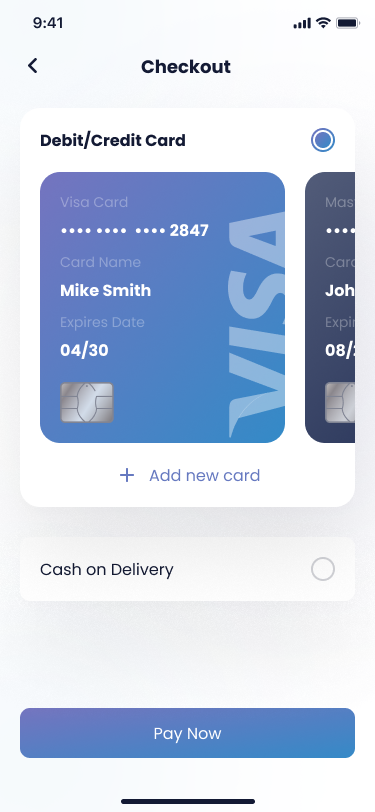
\includegraphics[width=\textwidth]{Images/Design/UIUX/renter/pay.png}
        \caption{Xác nhận \& Thanh toán}
    \end{subfigure}
    \caption{Quy trình đặt thuê xe (UC-04, UC-06)}
    \label{fig:ui-booking}
\end{figure}
Người dùng chọn thời gian thuê linh hoạt (tối thiểu 30 phút). Hệ thống AI gợi ý khung giờ “xanh” — khi xe ít được đặt và chủ xe đang online — giúp tăng tỷ lệ duyệt nhanh và giảm giá động. Màn hình thanh toán hiển thị rõ: phí thuê, phí nền tảng, tiền đặt cọc (hoàn lại 100\% nếu không hư hỏng), tổng tiền. Hỗ trợ nhiều phương thức: ví MoMo, ZaloPay, VNPay, thẻ tín dụng. Quy trình chỉ 3 bước, thời gian hoàn tất trung bình dưới 45 giây theo kết quả kiểm thử người dùng.
% \subsubsection*{4. Trong chuyến đi \& Trả xe}

% \begin{figure}[H]
%     \centering
%     \begin{subfigure}[b]{0.32\textwidth}
%         \centering
%         \includegraphics[width=\textwidth]{Images/UI/active_trip.png}
%         \caption{Theo dõi chuyến đi realtime}
%     \end{subfigure}
%     \hfill
%     \begin{subfigure}[b]{0.32\textwidth}
%         \centering
%         \includegraphics[width=\textwidth]{Images/UI/return_confirm.png}
%         \caption{Xác nhận trả xe}
%     \end{subfigure}
%     \hfill
%     \begin{subfigure}[b]{0.32\textwidth}
%         \centering
%         \includegraphics[width=\textwidth]{Images/UI/review.png}
%         \caption{Đánh giá sau chuyến}
%     \end{subfigure}
%     \caption{Theo dõi và kết thúc chuyến (UC-05, UC-07)}
%     \label{fig:ui-trip}
% \end{figure
\newpage
\subsubsection{Quản lý xe (dành cho chủ xe)}

\begin{figure}[H]
    \centering
    \begin{subfigure}[b]{0.32\textwidth}
        \centering
        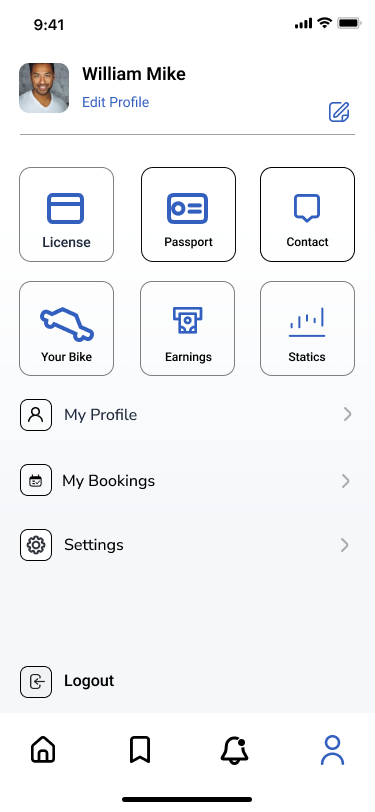
\includegraphics[width=\textwidth]{Images/Design/UIUX/owner/profile.png}
        \caption{Hồ sơ chủ xe}
    \end{subfigure}
    \hfill
    \begin{subfigure}[b]{0.32\textwidth}
        \centering
        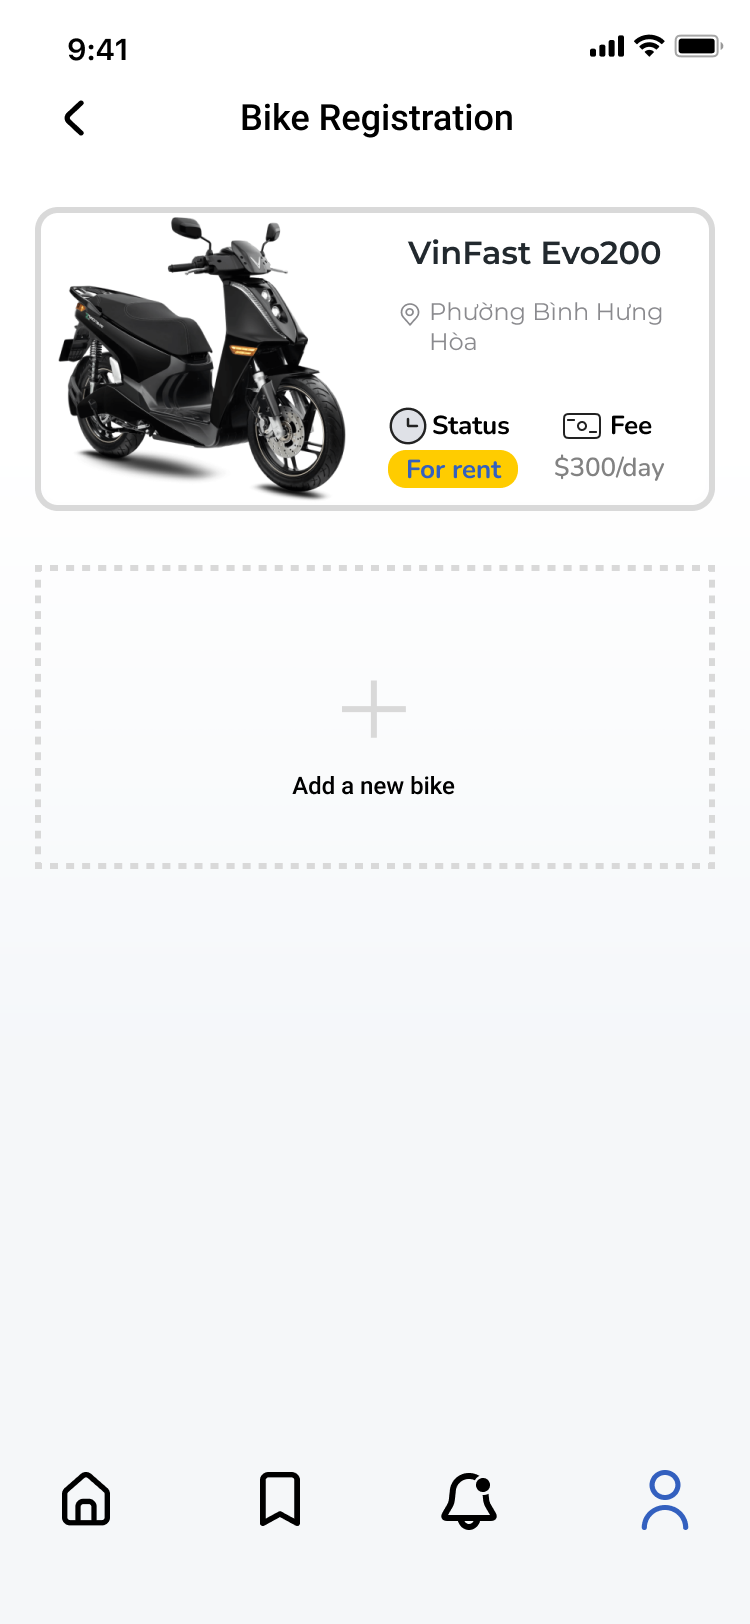
\includegraphics[width=\textwidth]{Images/Design/UIUX/owner/my-bike.png}
        \caption{Danh sách xe của tôi}
    \end{subfigure}
    \hfill
    \begin{subfigure}[b]{0.32\textwidth}
        \centering
        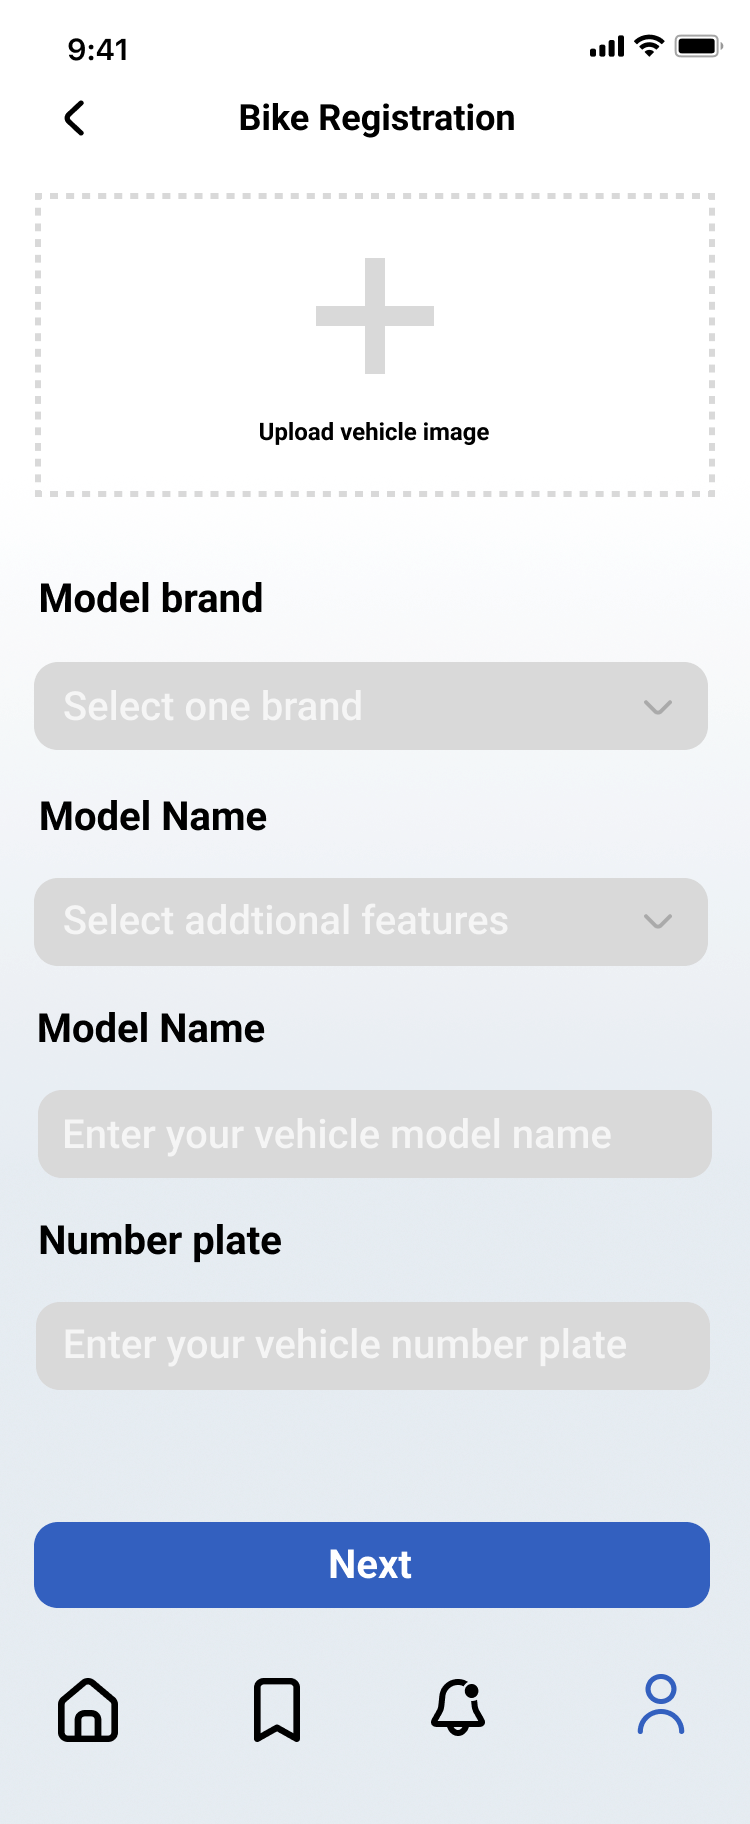
\includegraphics[width=\textwidth]{Images/Design/UIUX/owner/add.png}
        \caption{Đăng ký xe mới}
    \end{subfigure}
        \caption{Quản lý xe và thu nhập (UC-08, UC-09, UC-15)}

    \label{fig:ui-owner}
\end{figure}
Chủ xe có thể thêm xe mới chỉ trong 2 phút với các trường bắt buộc: biển số, hình ảnh 360°, giấy đăng ký xe. Màn hình danh sách xe hiển thị trạng thái realtime (khả dụng / đang thuê / bảo trì) và mức pin. Phần thu nhập thể hiện biểu đồ doanh thu theo ngày/tuần/tháng, tỷ lệ sử dụng xe giúp chủ xe tối ưu thời gian cho thuê.
% \subsubsection*{6. Dashboard quản trị viên (Web Admin – React.js)}

% \begin{figure}[H]
%     \centering
%     \begin{subfigure}[b]{0.45\textwidth}
%         \centering
%         \includegraphics[width=\textwidth]{Images/UI/admin_dashboard.png}
%         \caption{Tổng quan hệ thống}
%     \end{subfigure}
%     \hfill
%     \begin{subfigure}[b]{0.45\textwidth}
%         \centering
%         \includegraphics[width=\textwidth]{Images/UI/admin_vehicle_approval.png}
%         \caption{Duyệt xe chờ}
%     \end{subfigure}
%     \caption{Giao diện quản trị web}
%     \label{fig:ui-admin}
% \end{figure}

% Tất cả giao diện đều được thiết kế responsive, hỗ trợ chế độ tối (dark mode), tiết kiệm pin và dữ liệu di động theo yêu cầu phi chức năng đã nêu ở mục \ref{fig:non-functional}.